\section{Přehled}

Dnešní verze elektronického trezoru se zamyká pomocí mechanizmu bajonetu a~magneticky řízené zpětné západky. 

\begin{figure}[h]
    \centering
    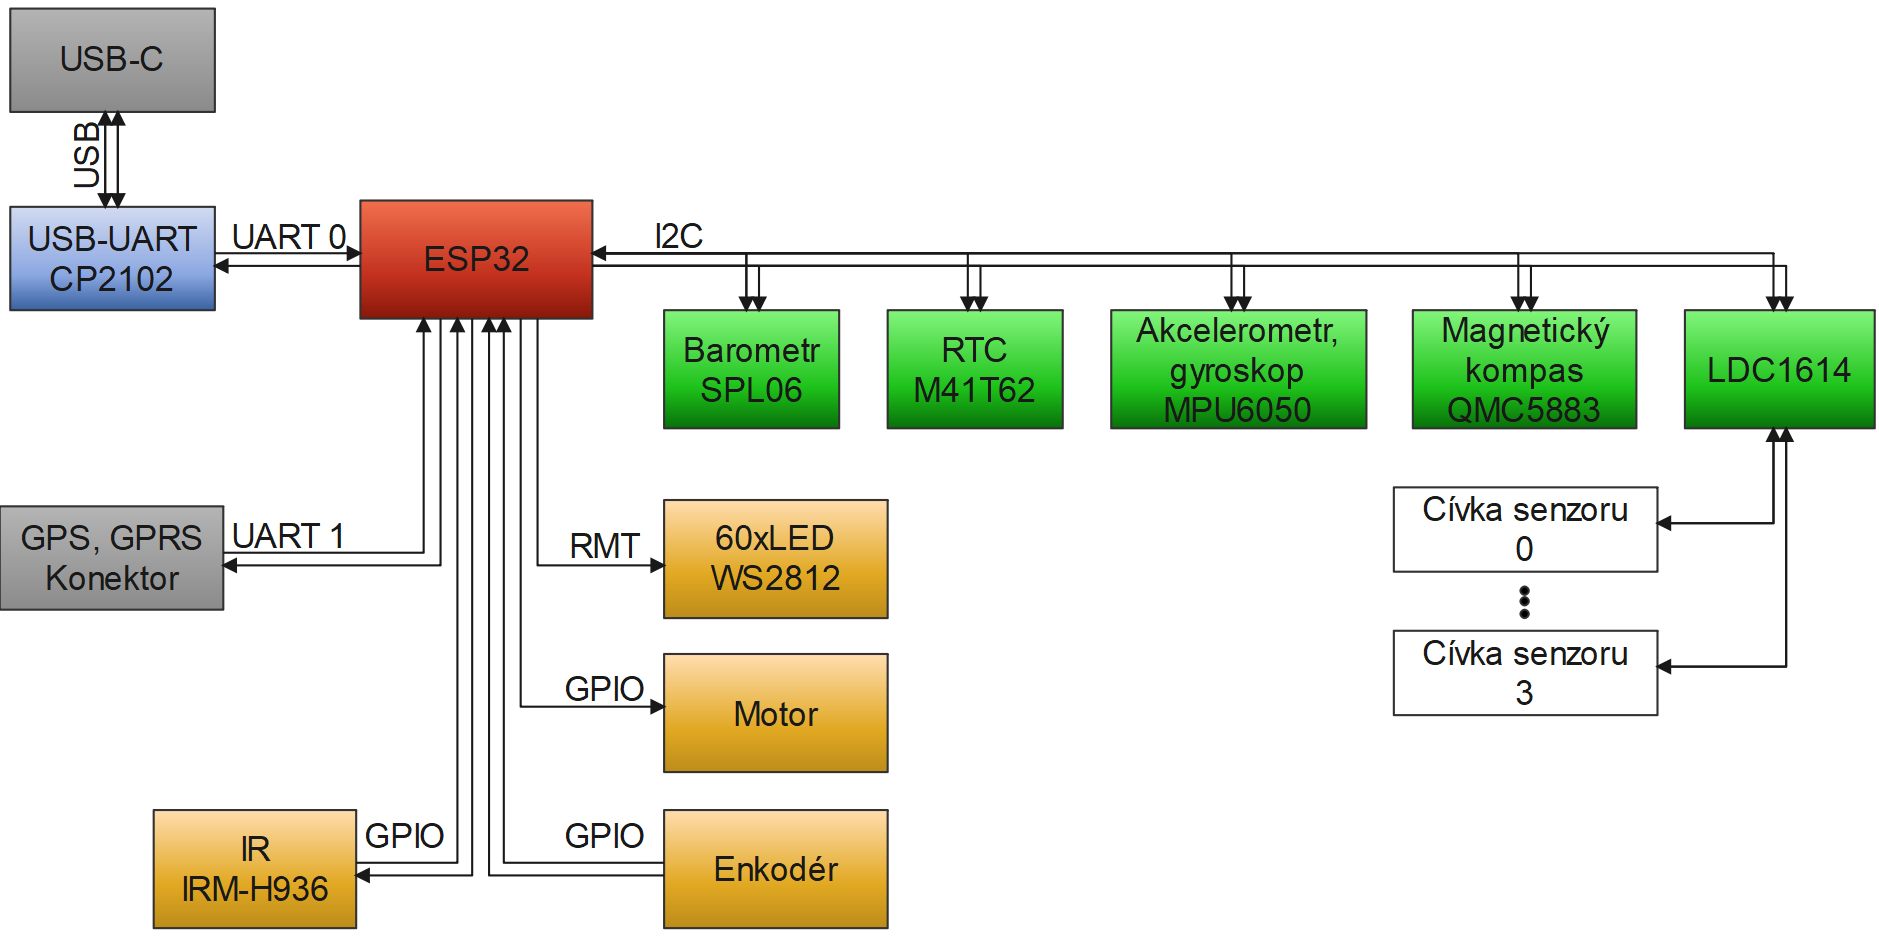
\includegraphics[width=\textwidth]{kapitoly/obrazky/E4/uvod/logika.png}
    \caption{Blokové schéma logických částí BlackBoxu}
    \label{fig:E4-Blokovka_logika}
\end{figure}

Elektronika je vybavena čipem ESP32 \parencite{ESP32}, \parencite{ESP32-WROVER-B},
který obsahuje dva procesory Xtensa LX6, WiFi a~bluetooth. Dále je trezor vybaven čipem BMX055 \parencite{bmx055} nebo dvojicí čipů MPU6050 \parencite{mpu6050} 
a~QMC5883 \parencite{qmc5883}, které poskytují gyroskop, akcelerometr a~magnetický kompas. 
Dále je zde SPL06 \parencite{spl06}, barometr s~rozlišením 0,06~hPa, který umožňuje rozeznat změnu nadmořské výšky 
o~polovinu metru. Další systém trezoru je možnost IR komunikace, která je zde pro možnost jednoznačné identifikace dveří, ale pochopitelně může 
sloužit i~pro jiný účel. Deska je také vybavena RTC a~má vlastní programátor pro usnadnění programování. Vedle ESP32 je zde asi 
nejvýznamnějším čipem LDC1614 \parencite{LDC1614}, případně LDC1314, který umožňuje funkci tlakové plochy (viz kapitoly \ref{E4-mech_tlakovky}, \ref{E4-tlakovka}).

%todo doplnit popis a využití a možnosti tlakové desky 

\begin{table}[h]
    \centering
    \resizebox{\textwidth}{!}{%
    \begin{tabular}{@{}lll@{}} 
    \textbf{čip} & \textbf{popis} & \textbf{poznámky}
                                                                                    \\ \midrule
    \textbf{ESP32}              & dve jádra Xtensa LX6, WiFi a~bluetooth        &                                                   \\
    \textbf{BMX055}             & gyroskop, akcelerometr, magnetický kompas     & možno nahradit dvojicí čipů MPU6050 a~QMC5883     \\
    \textbf{SPL06}              & barometr                                      & rozlišení až 0,06~hPa                              \\
    \textbf{IRM-H936 a~IR led}  & IR komunikace                                 &                                                   \\
    \textbf{LDC1614}            & snímání tlakové desky                         & počítá se s~možnou záměnou za LDC1314             \\
    \textbf{CP2102}             & programátor                                   & s~hardwarově zajištěným odpojováním napájení      \\ \bottomrule
    \end{tabular}%
    }
    \caption{Shrnutí elektronického vybavení}
    \label{tab:shrnuti}
\end{table}


% Na tomto Blokovém schéma i můžete udělat obrázek o zapojení jednotlivých čipu a jiných logických obvodů.
% Můžete si všimnout sběrnice I2C kterou využívají senzory jako gyroskop, magnetický kompas, barometr nebo 
% tlaková plocha která je reprezentována čipem LDC1614.
% Dále si můžete všimnout že světelný kruh přebírá od ESP informace pomocí periferie RMT 

\newpage